\subsection{Dinâmica da base e torques de controle}
\label{sec:cap4_app_final_base_torques}

A dinâmica da base durante a aproximação final pode ser sintetizada pelas faixas de variação e pelos valores finais das velocidades e acelerações angulares combinadas dos modos de Euler e Lagrange.

\subsubsection{Velocidade angular da base robótica}

A Tabela~\ref{tab:cap4_vel_base} resume as componentes da velocidade angular da base ao longo da simulação, enquanto a Figura~\ref{fig:cap4_app_final_veloc_base} ilustra o comportamento temporal desses sinais.

\begin{table}[H]
\centering
\caption{Faixas e valores finais das velocidades angulares da base.}
\label{tab:cap4_vel_base}
\begin{tabularx}{\linewidth}{|
  >{\centering\arraybackslash}X|
  >{\centering\arraybackslash}X|
  >{\centering\arraybackslash}X|}
\hline
\textbf{Componente} &
\textbf{Faixa ao longo da simulação [rad/s]} &
\textbf{Valor final [rad/s]} \\
\hhline{|=|=|=|}
$w_x$ & $-1{,}20 \text{ a } 1{,}20$ & $0{,}01$ \\
\hline
$w_y$ & $-1{,}26 \text{ a } 1{,}25$ & $-0{,}01$ \\
\hline
$w_z$ & $-0{,}96 \text{ a } 1{,}00$ & $0{,}03$ \\
\hline
\end{tabularx}
\end{table}

\begin{figure}[H]
\centering

\includegraphics[width=1.0\linewidth]{4 Resultados e discussoes/Imagens/3 App final/2a Veloc angular base Euler Lagrange.png}
\caption{Velocidades angulares da base combinando as fases em Euler e Lagrange.}
\label{fig:cap4_app_final_veloc_base}
\end{figure}

\subsubsection{Aceleração angular da base robótica}

A Tabela~\ref{tab:cap4_acel_base} apresenta as acelerações angulares correspondentes. Os picos se concentram na região de transição entre as dinâmicas e durante a atuação mais intensa do controlador, mas os valores finais retornam para níveis compatíveis com ajustes finos de atitude na vizinhança da porta de acoplamento.

\begin{table}[H]
\centering
\caption{Faixas e valores finais das acelerações angulares da base.}
\label{tab:cap4_acel_base}
\begin{tabularx}{\linewidth}{|
  >{\centering\arraybackslash}X|
  >{\centering\arraybackslash}X|
  >{\centering\arraybackslash}X|}
\hline
\textbf{Componente} &
\textbf{Faixa ao longo da simulação [rad/s$^2$]} &
\textbf{Valor final [rad/s$^2$]} \\
\hhline{|=|=|=|}
$\dot{w}_x$ & $-57{,}64 \text{ a } 3{,}50$  & $2{,}00$ \\
\hline
$\dot{w}_y$ & $-109{,}9 \text{ a } 6{,}48$ & $2{,}00$ \\
\hline
$\dot{w}_z$ & $-61{,}73 \text{ a } 3{,}55$ & $-2{,}00$ \\
\hline
\end{tabularx}
\end{table}

\begin{figure}[H]
\centering
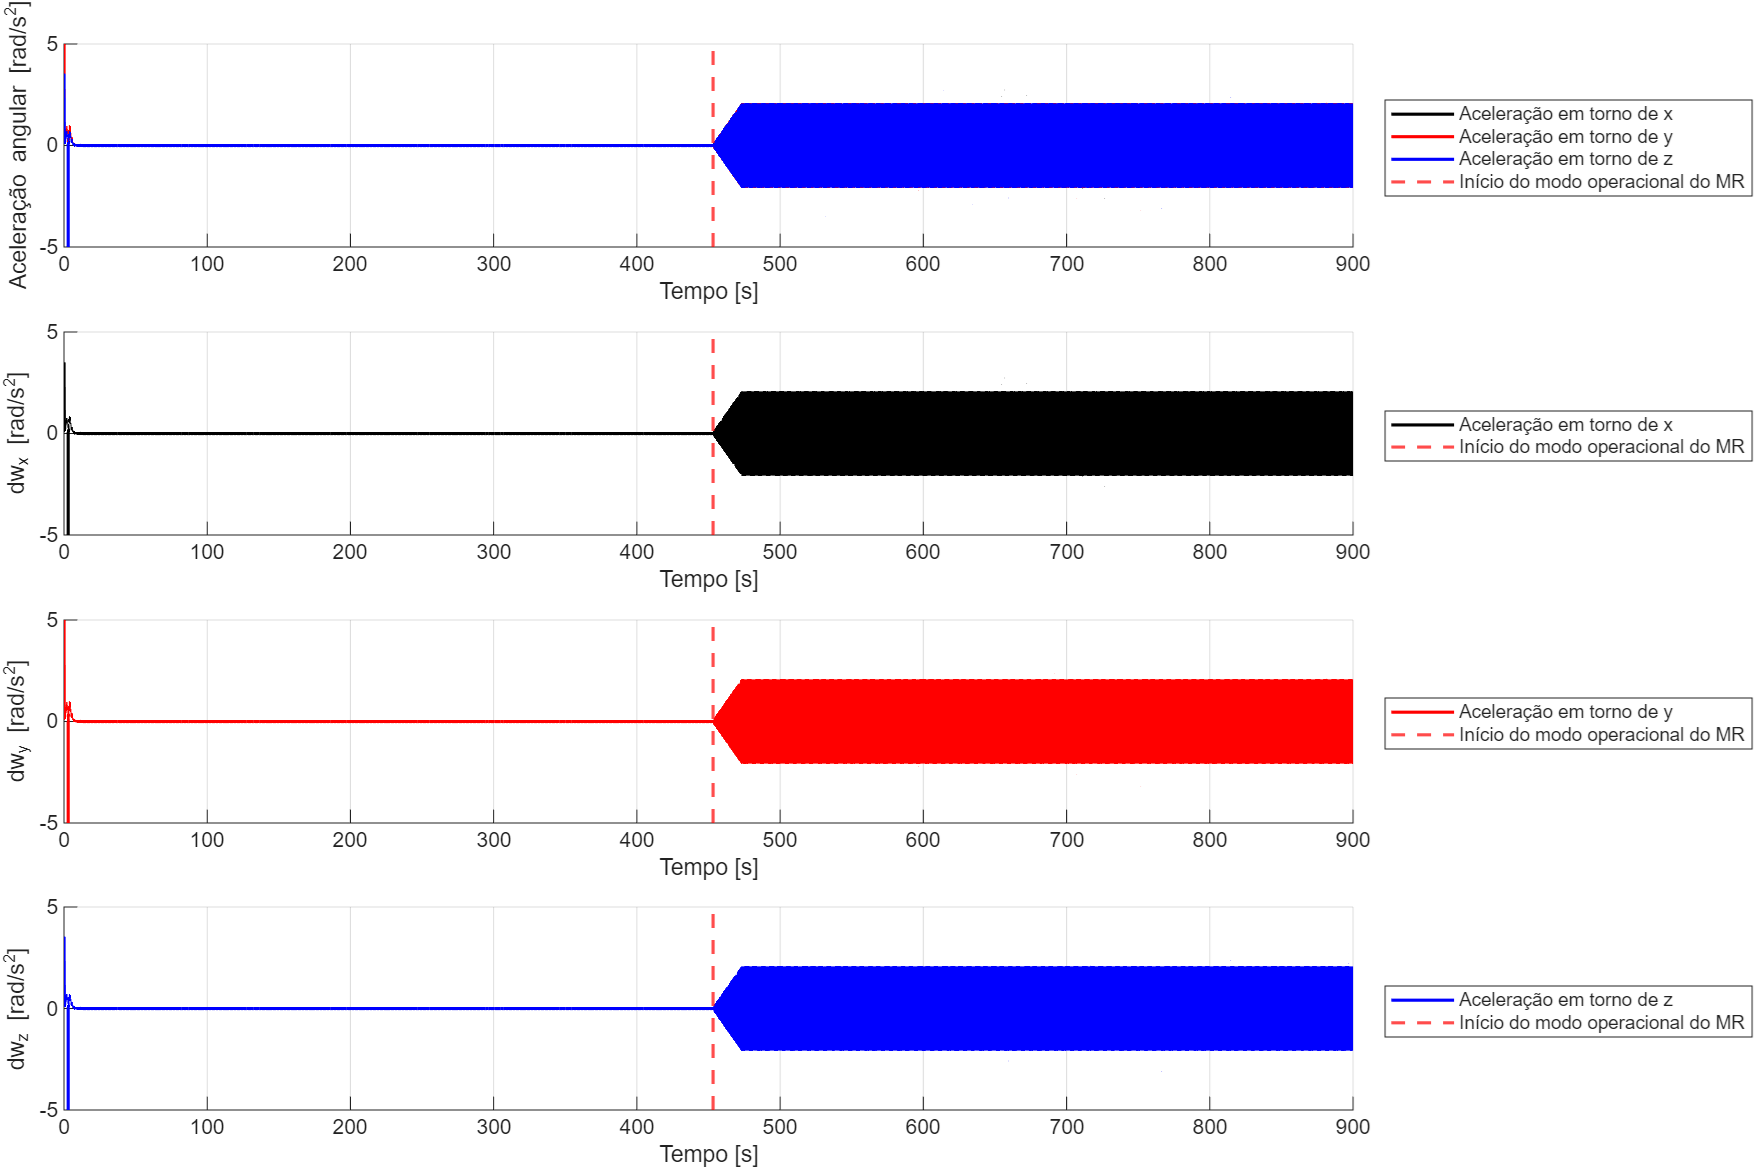
\includegraphics[width=1.0\linewidth]{4 Resultados e discussoes/Imagens/3 App final/2b Acel angular base Euler Lagrange.png}
\caption{Acelerações angulares da base na transição entre os modos de operação.}
\label{fig:cap4_app_final_acel_base}
\end{figure}

As Figuras~\ref{fig:cap4_app_final_veloc_base} e \ref{fig:cap4_app_final_acel_base} mostram que, ao longo da aproximação final, as velocidades angulares da base permanecem em faixas moderadas e as acelerações concentram seus picos na região de transição entre os modos de Euler e Lagrange. Após esses transitórios, observa-se que a base evolui para uma condição de rotação lenta, com variações angulares e acelerações residuais.

\subsubsection{Torque de controle de atitude da base robótica}

\begin{figure}[H]
\centering
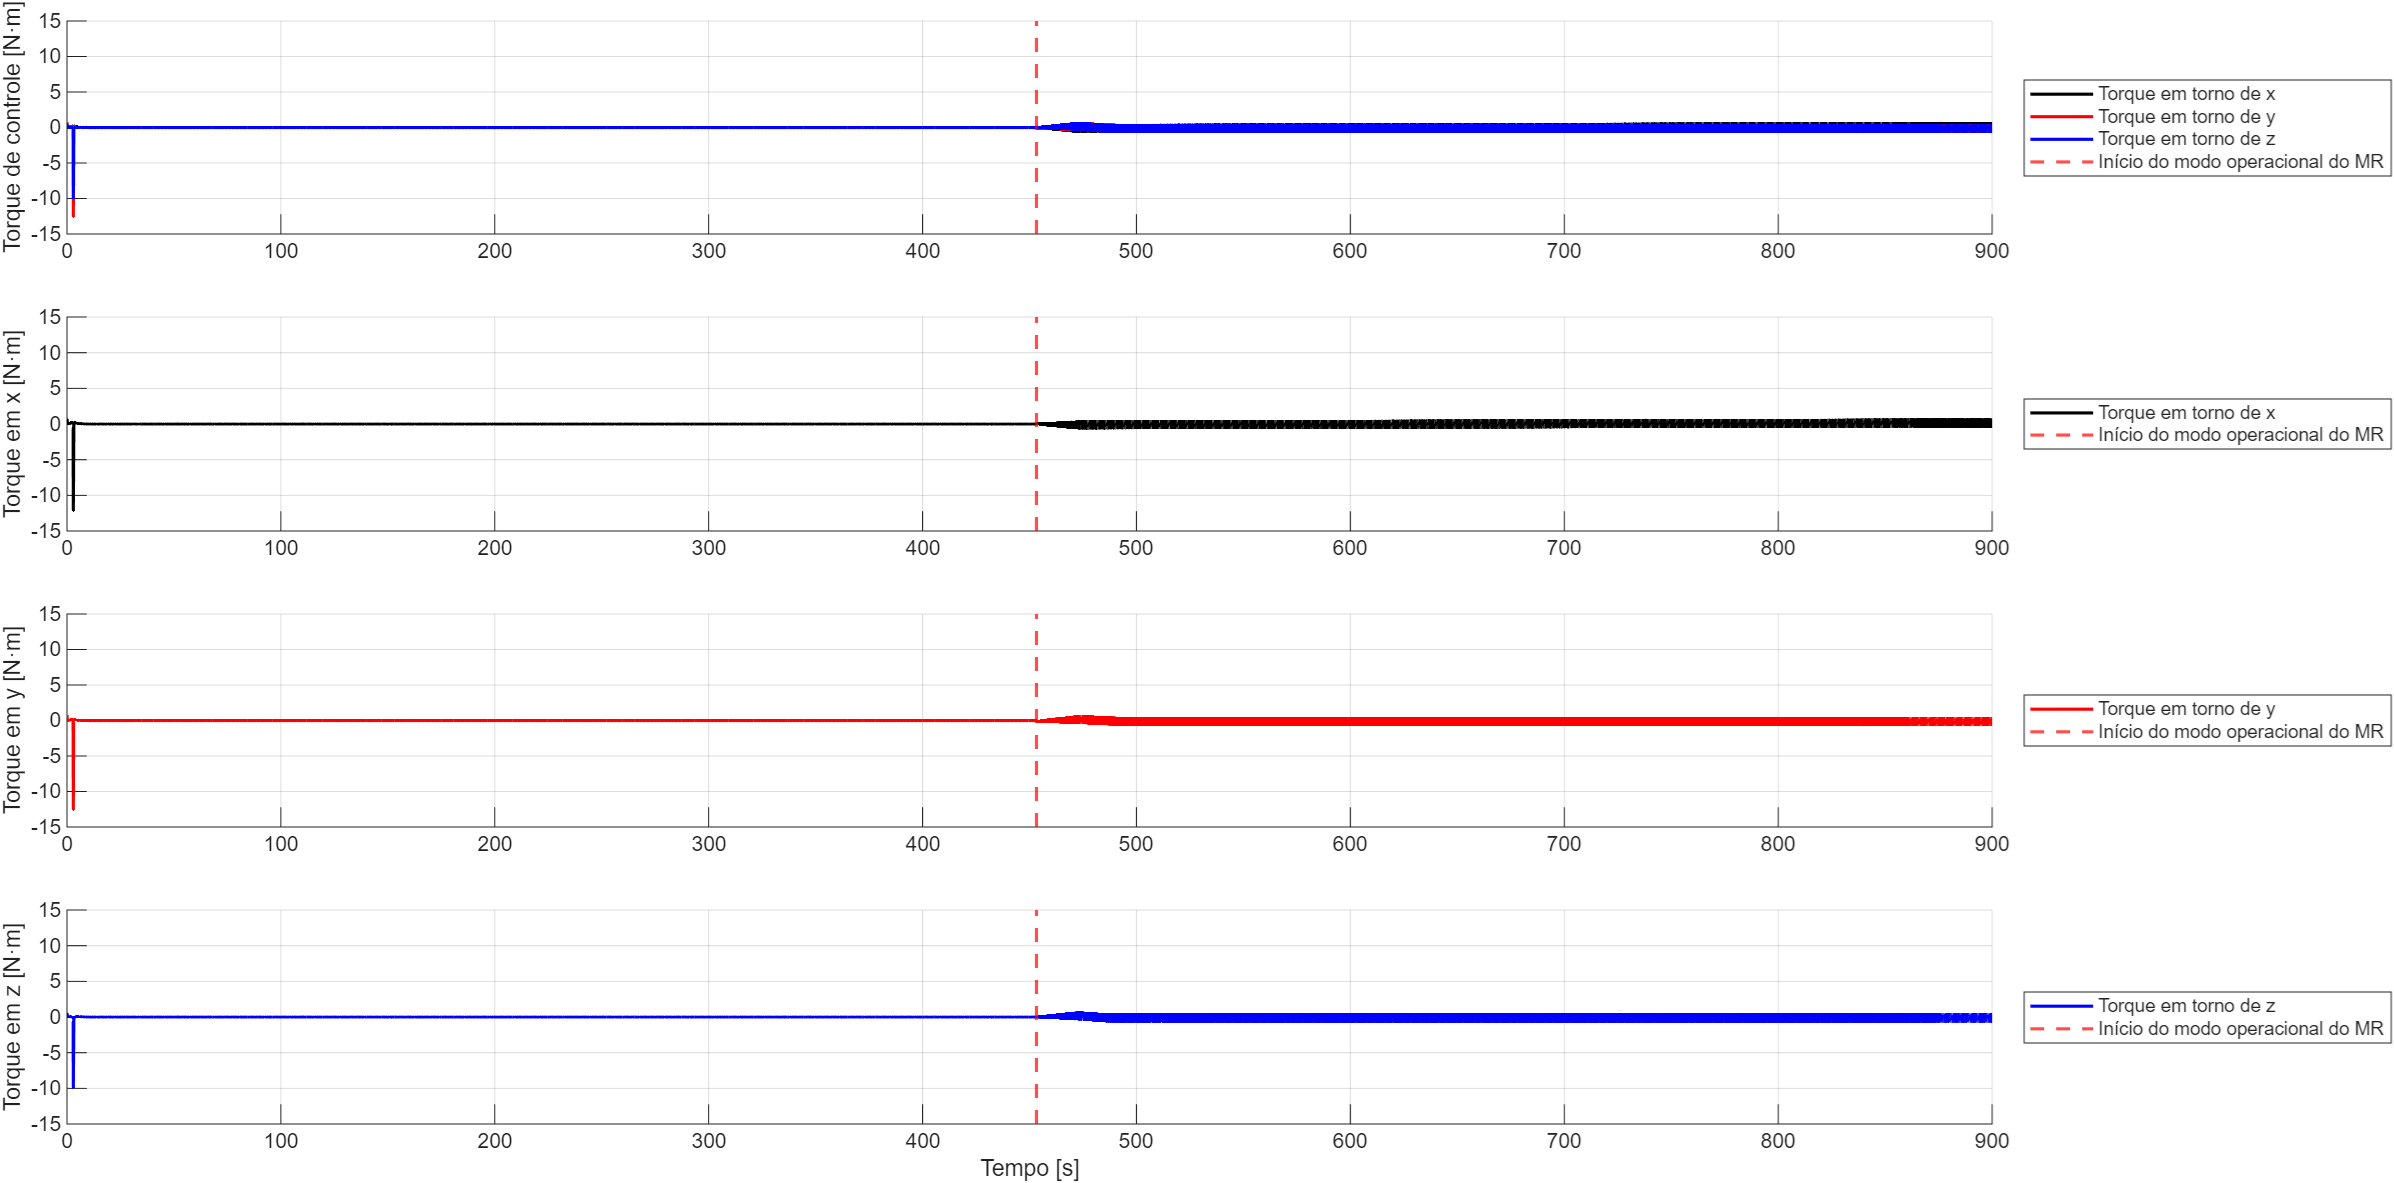
\includegraphics[width=1.0\linewidth]{4 Resultados e discussoes/Imagens/3 App final/3a Torque de controle.png}
\caption{Torques de controle de atitude aplicados pelo controlador PD.}
\label{fig:cap4_app_final_torque_controle}
\end{figure}

A atuação do controlador de atitude é sintetizada na Figura~\ref{fig:cap4_app_final_torque_controle}, que apresenta as componentes do torque PD aplicadas à base. As faixas de variação e os valores finais desses torques estão resumidos na Tabela~\ref{tab:cap4_torque_PD}. Nota-se que o esforço de controle possui torques finais próximos de zero nos eixos $x$ e $y$ e um valor residual mais pronunciado em $z$, associado ao eixo de controle dominante, pois é o eixo em que o \gls{mr} mais se movimenta para alcançar a porta de acoplamento.

\begin{table}[H]
\centering
\caption{Faixas e valores finais dos torques de controle de atitude (PD).}
\label{tab:cap4_torque_PD}
\begin{tabularx}{\linewidth}{|
  >{\centering\arraybackslash}X|
  >{\centering\arraybackslash}X|
  >{\centering\arraybackslash}X|}
\hline
\textbf{Componente} &
\textbf{Faixa ao longo da simulação [N·m]} &
\textbf{Valor final [N·m]} \\
\hhline{|=|=|=|}
$\tau_x$ & $-12{,}07 \text{ a } 0{,}74$ & $-0{,}016$ \\
\hline
$\tau_y$ & $-12{,}49 \text{ a } 0{,}74$ & $0{,}028$ \\
\hline
$\tau_z$ & $-9{,}88 \text{ a } 0{,}61$  & $-0{,}58$ \\
\hline
\end{tabularx}
\end{table}

\subsubsection{Compensação do acoplamento dinâmico}

A versão compensada do torque de controle, que inclui termos de compensação dos acoplamentos dinâmicos entre base e manipulador, é apresentada na Figura~\ref{fig:cap4_app_final_torque_compensado}. Os valores finais, reunidos na Tabela~\ref{tab:cap4_torque_PD_comp}, são muito próximos aos do torque PD puro, com diferenças da ordem de $10^{-3}$ a $10^{-2}$ N·m. Isso indica que, para o cenário considerado, a compensação influencia principalmente a forma transitória, sem alterar de modo significativo o nível de esforço requerido em regime quase estacionário.

\begin{figure}[H]
\centering
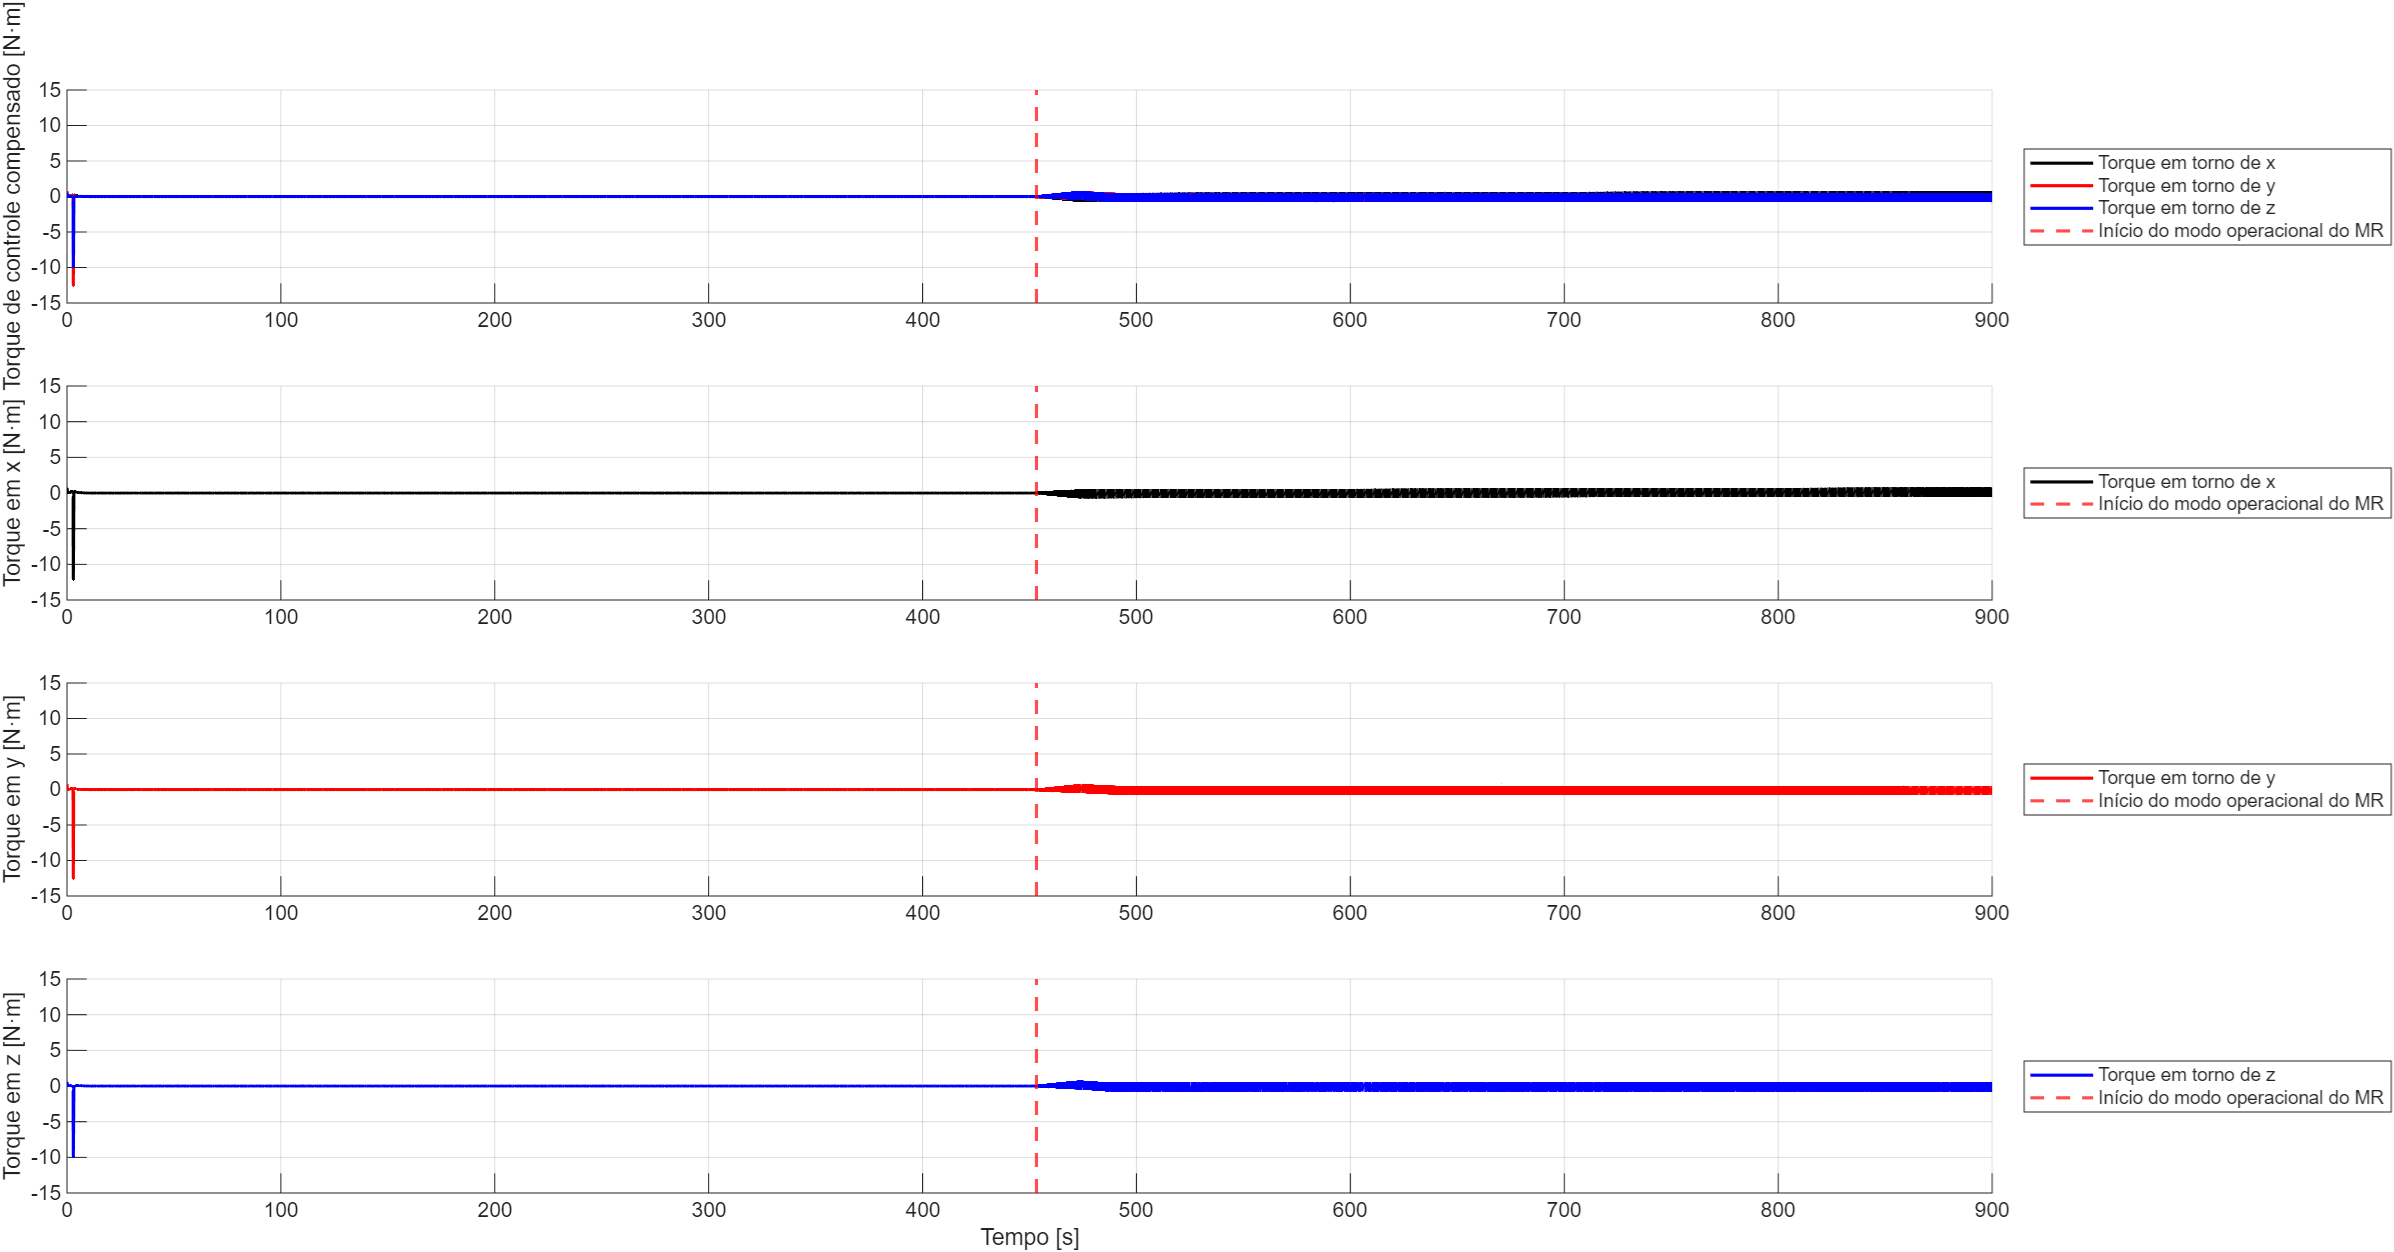
\includegraphics[width=1.0\linewidth]{4 Resultados e discussoes/Imagens/3 App final/3c Torque compensado.png}
\caption{Torques de controle de atitude com compensação dos efeitos do manipulador.}
\label{fig:cap4_app_final_torque_compensado}
\end{figure}

\begin{table}[H]
\centering
\caption{Valores finais dos torques de controle compensados.}
\label{tab:cap4_torque_PD_comp}
\begin{tabularx}{\linewidth}{|
  >{\centering\arraybackslash}X|
  >{\centering\arraybackslash}X|}
\hline
\textbf{Componente} &
\textbf{Valor final [N·m]} \\
\hhline{|=|=|}
$\tau_x^{\text{comp}}$ & $-0{,}023$ \\
\hline
$\tau_y^{\text{comp}}$ & $0{,}024$ \\
\hline
$\tau_z^{\text{comp}}$ & $-0{,}59$ \\
\hline
\end{tabularx}
\end{table}

\subsubsection{Torques de reação da base robótica}

O efeito direto da movimentação do manipulador sobre a base é avaliado por meio dos torques de reação ilustrados na Figura~\ref{fig:cap4_app_final_torque_reacao}. As faixas de variação e os valores finais são apresentados na Tabela~\ref{tab:cap4_torque_reacao}. Observa-se que esses torques permanecem significativamente abaixo dos torques de controle, reforçando que as perturbações induzidas pelo manipulador são eficazmente rejeitadas pelo sistema de atitude e pela própria inércia da estrutura.

\begin{figure}[H]
\centering
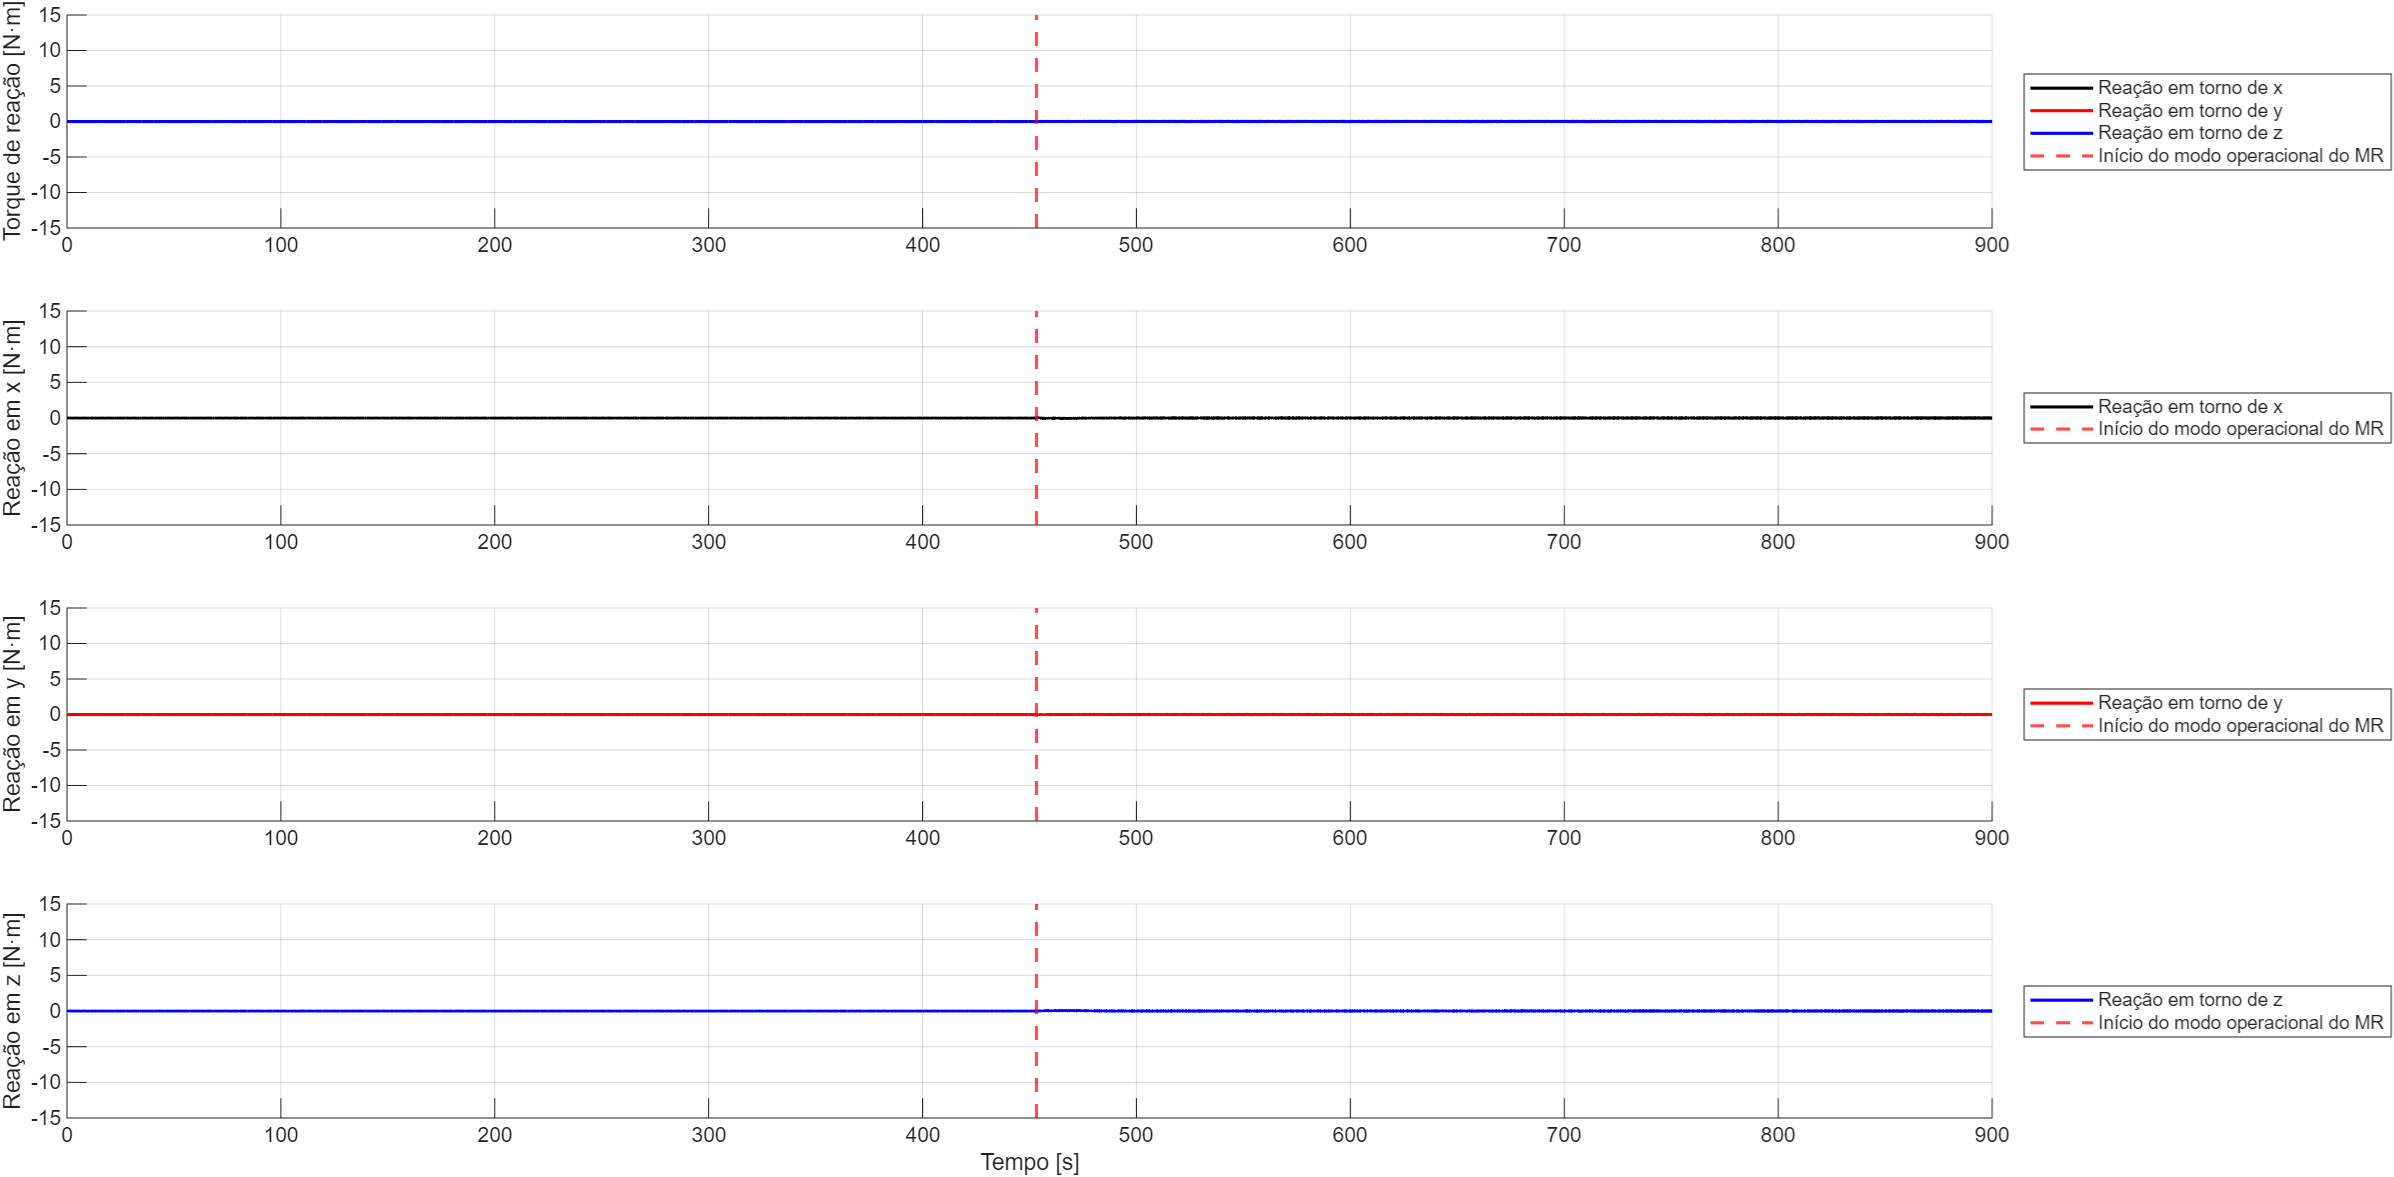
\includegraphics[width=1.0\linewidth]{4 Resultados e discussoes/Imagens/3 App final/3b Torque reacao.png}
\caption{Torques de reação na base decorrentes do movimento do manipulador.}
\label{fig:cap4_app_final_torque_reacao}
\end{figure}

\begin{table}[H]
\centering
\caption{Faixas e valores finais dos torques de reação na base.}
\label{tab:cap4_torque_reacao}
\begin{tabularx}{\linewidth}{|
  >{\centering\arraybackslash}X|
  >{\centering\arraybackslash}X|
  >{\centering\arraybackslash}X|}
\hline
\textbf{Componente} &
\textbf{Faixa ao longo da simulação [N·m]} &
\textbf{Valor final [N·m]} \\
\hhline{|=|=|=|}
$\tau_x^{\text{reac}}$ & $-0{,}0206 \text{ a } 0{,}0309$ & $0{,}0066$ \\
\hline
$\tau_y^{\text{reac}}$ & $-0{,}0704 \text{ a } 0{,}0132$ & $0{,}0039$ \\
\hline
$\tau_z^{\text{reac}}$ & $-0{,}0051 \text{ a } 0{,}0300$ & $0{,}0051$ \\
\hline
\end{tabularx}
\end{table}

\subsubsection{Energia cinética}

A coerência entre os resultados de torque e a resposta global do sistema pode ser verificada na Figura~\ref{fig:cap4_app_final_energia_cinetica}, que apresenta a evolução da energia cinética da base, dos elos e do sistema como um todo. Os valores máximos e finais dessas energias são sintetizados na Tabela~\ref{tab:cap4_energia_cinetica}. Verifica-se que, após os transitórios, tanto a energia da base quanto a dos elos se reduzem a níveis muito baixos, caracterizando um regime de movimento quase estacionário ao final da aproximação.

\begin{figure}[H]
\centering
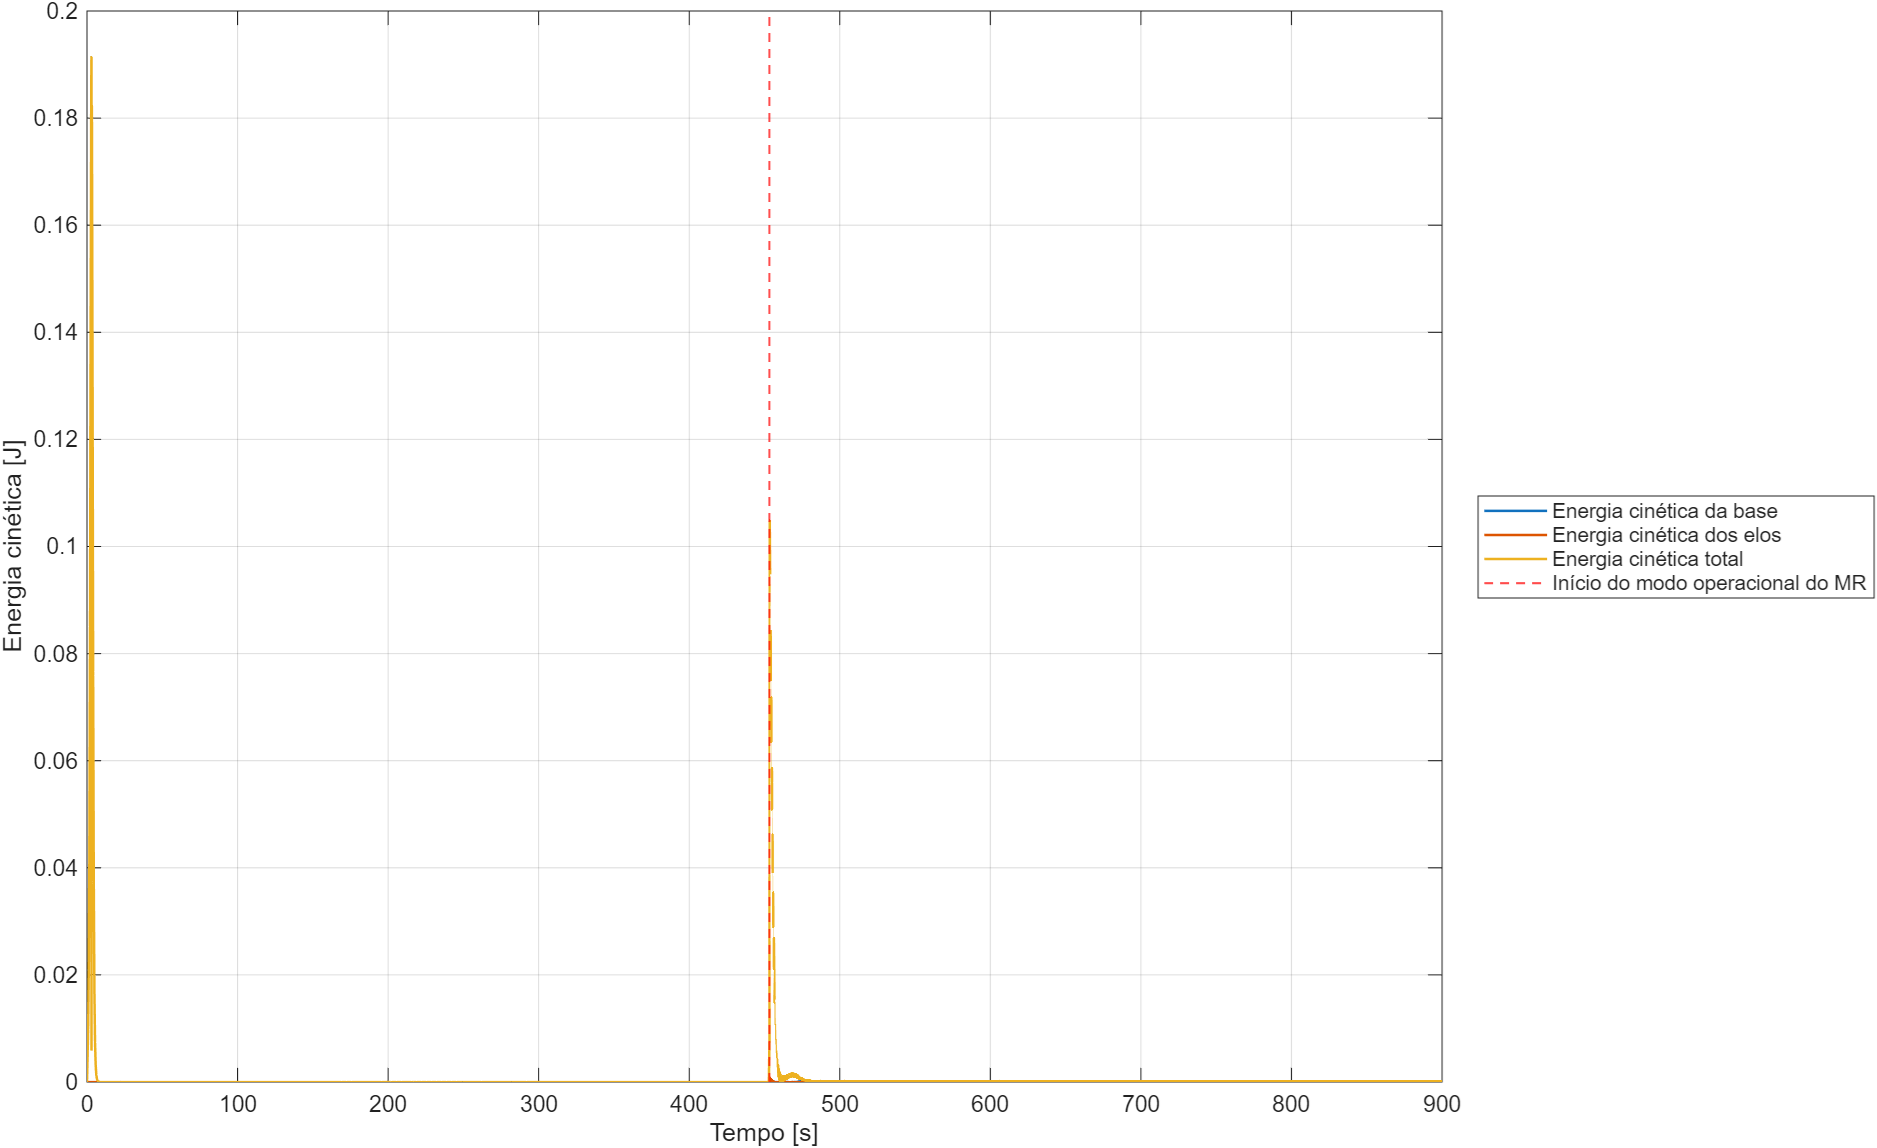
\includegraphics[width=1.0\linewidth]{4 Resultados e discussoes/Imagens/3 App final/6 Energia cinetica.png}
\caption{Energia cinética da base, dos elos e total do sistema ao longo da aproximação final.}
\label{fig:cap4_app_final_energia_cinetica}
\end{figure}

\begin{table}[H]
\centering
\caption{Valores máximos e finais das energias cinéticas.}
\label{tab:cap4_energia_cinetica}
\begin{tabularx}{\linewidth}{|
  >{\centering\arraybackslash}X|
  >{\centering\arraybackslash}X|
  >{\centering\arraybackslash}X|}
\hline
\textbf{Grandeza} &
\textbf{Valor máximo [J]} &
\textbf{Valor final [J]} \\
\hhline{|=|=|=|}
$E_{\text{base}}$ & $0{,}1914$ & $7{,}313\times 10^{-5}$ \\
\hline
$E_{\text{elos}}$ & $9{,}326\times 10^{-4}$ & $1{,}704\times 10^{-7}$ \\
\hline
$E_{\text{tot}}$  & 0{,}1914 & $1{,}349\times 10^{-4}$ \\
\hline
\end{tabularx}
\end{table}

\subsubsection{Momento angular}
As componentes do momento angular total (base + elos) permanecem confinadas em intervalos estreitos ao longo dos $900$ s de simulação, com amplitudes máximas da ordem de $10^{-1}$ N·m·s e valores finais na faixa de $10^{-3}$–$10^{-2}$ N·m·s. A Tabela~\ref{tab:cap4_momento_angular} sintetiza as faixas observadas e os valores residuais ao final da aproximação, evidenciando que o sistema encerra a fase de acoplamento com baixa quantidade de movimento angular armazenada.

\begin{table}[H]
\centering
\caption{Faixas e valores finais das componentes do momento angular total.}
\label{tab:cap4_momento_angular}
\begin{tabularx}{\linewidth}{|
  >{\centering\arraybackslash}X|
  >{\centering\arraybackslash}X|
  >{\centering\arraybackslash}X|}
\hline
\textbf{Componente} &
\textbf{Faixa ao longo da simulação [N·m·s]} &
\textbf{Valor final [N·m·s]} \\
\hhline{|=|=|=|}
$h_x$ & $-0{,}09494 \text{ a } 0{,}09511$ & $0{,}00236$ \\
\hline
$h_y$ & $-0{,}1415 \text{ a } 0{,}0990$ & $-0{,}00504$ \\
\hline
$h_z$ & $-0{,}1426 \text{ a } 0{,}1452$ & $0{,}01513$ \\
\hline
\end{tabularx}
\end{table}


Em conjunto, as Figuras~\ref{fig:cap4_app_final_veloc_base}--\ref{fig:cap4_app_final_energia_cinetica} e as Tabelas~\ref{tab:cap4_torque_PD}--\ref{tab:cap4_momento_angular} indicam que o sistema encerra a aproximação final em uma condição de baixa energia cinética, baixo momento angular residual e níveis moderados de torque de controle, com torques de reação significativamente menores.